\chapter{Radar Theory}\label{chap:Radar Theory}
Radar technology is a broad field,  and aspects of radar theory covered below only hold significance to the audio radar and is not an attempt to reproduce a radar textbook but to aid in the understanding of the design process followed in Chapter \ref{chap:Methodology}.
\section{Principles of Radar Operation}
\subsection{Range Concepts}
To measure range with radar, the speed of type of signal through the medium it is travelling needs to be considered. In the audio radar context, an audible signal travels through the atmosphere at a speed of $343\ m.s^{-1}$. A chirp\footnote{See section \ref{sec:chirp}} is transmitted out from an antenna (speaker) and then the receiver (microphone) listens for the return echo that would have reflected back after hitting the target. In order to measure the distance to the target, Equation \ref{eq:range} is used.
\begin{equation}
\tau = \frac{2R}{c}\label{eq:range}
\end{equation}
Where $\tau$ is the time delay between the start when the transmitting pulse was transmitted and the returning echo. $R$ is the range that to the target and it is multiplied by $2$ since the pulse travels to the target and back. The speed of sound is $c$. The range concept using the Equation \ref{eq:range} can be better explained using Figure \ref{fig:rangeConcept}.
\begin{figure}[h!]
    \centering
    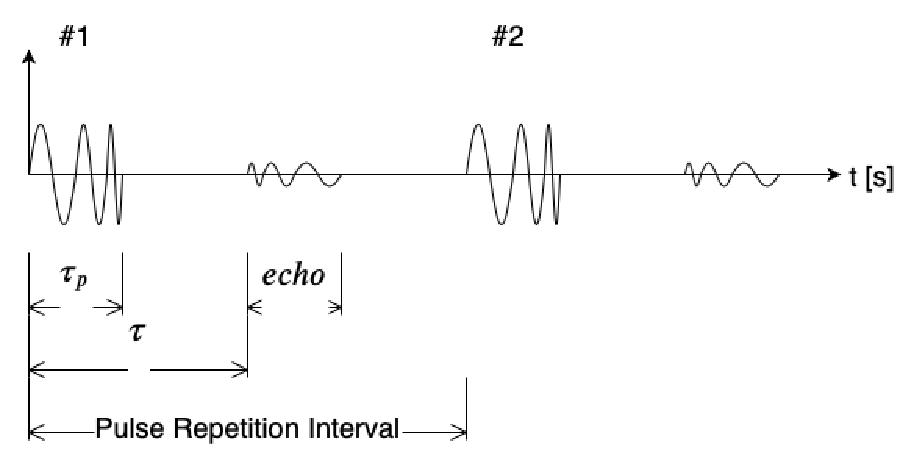
\includegraphics[width = 0.5\textwidth]{images/PRI.pdf}
    \caption{Pulse Repetition Interval\cite{richards_principles_2010}}\label{fig:PRI}
\end{figure}
\begin{figure}[h!]
    \centering
    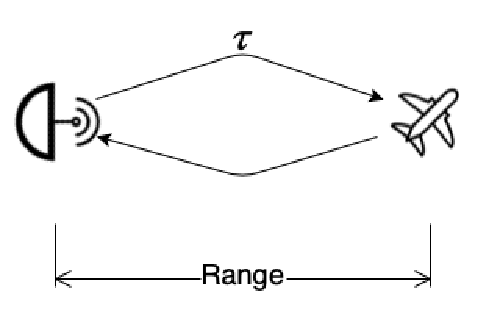
\includegraphics[width = 0.4\textwidth]{images/rangeConcept.pdf}
    \caption{Radar Range Concept \cite{richards_principles_2010}}\label{fig:rangeConcept}
\end{figure}

\subsection{Range Resolution}
Range resolution can be described as the minimum distance two or more targets need to be apart to be distinguishable from each other \cite{noauthor_radar_nodate}. If two targets are too close together, they will show up as a single object on the resulting range line. To better explain this concept, Figure \ref{fig:rangeRes} depicts the concept visually.

\begin{figure}[h!]
    \centering
    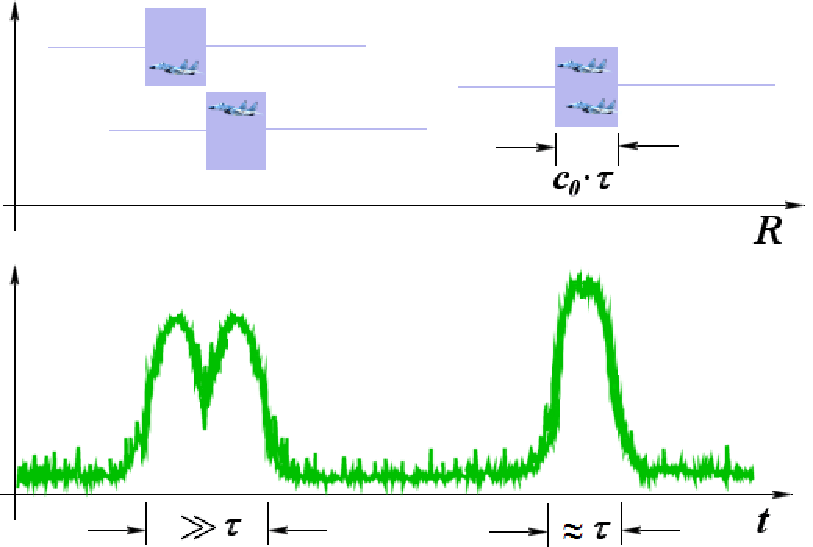
\includegraphics[width = 0.5\textwidth]{images/ra1.pdf}
    \caption{Range Resolution \cite{noauthor_radar_nodate}}\label{fig:rangeRes}
\end{figure}

The range resolution in Figure \ref{fig:rangeRes} shows that when the two fighter jets are flying above each other, they are perceived as a single target on the spike in the received signal.
Equation \ref{eq:rangeRes} governs the range resolution and is in terms of the speed of sound ($c$) \footnote{Working in audio spectrum} and the bandwidth ($B$) of the chirp. 
\begin{equation}
\Delta R = \frac{c}{2B}\label{eq:rangeRes}
\end{equation}
Where $\Delta R$ is the minimum distance that two objects can be apart to be able to detect them as two distinct targets.
\subsection{Unambiguous and Ambiguous Range}
The concept of the unambiguous and ambiguous range goes hand in hand with each other. The unambiguous range of a radar is the maximum distance that a transmitted pulse can travel to a target and back before the next pulse is transmitted \cite{noauthor_radar_nodate-1}. In Figure \ref{fig:rangeU}, the echo is only received after the second pulse is transmitted. The radar would consider this echo to be associated with a target much closer than in actuality.
\begin{figure}[h!]
    \centering
    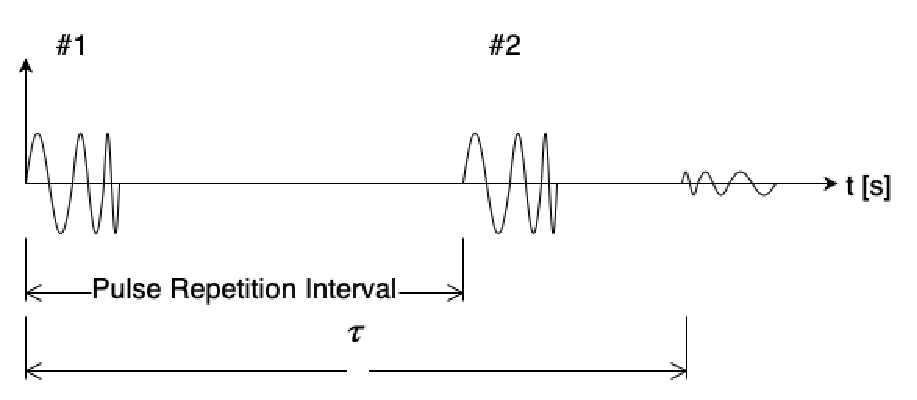
\includegraphics[width = 0.5\textwidth]{images/RangeU.pdf}
    \caption{Unambiguous Range}\label{fig:rangeU}
\end{figure}
To calculate the maximum range that the radar can detect a target unambiguously Equation \ref{eq:rangeU} is used. Consider Figure \ref{eq:rangeU}, and assume a target $225\ m$ away\footnote{Using Equation \ref{eq:range}} with $\tau\ =\ 1.312\ s $ and $PRI\ =\ 1\ s$

\begin{equation}
\begin{align*}
R_u = \frac{c}{2PRF}\\ = \frac{343}{2(1)}\\
= 171.5\ m\\ \label{eq:rangeU}
\end{align*}
\end{equation}
In actual fact the radar perceives the target to be at $225\ m - 171.5\ m\ =\ \textbf{53.5 m}$which can be classified as the ambiguous range of the radar.
\subsection{Doppler Frequency and Effect}
Doppler Frequency can be obtained from the phenomenon of the Doppler Effect discovered by Christian Doppler \cite{noauthor_radar_nodate-2}. The Doppler Effect is the perceived change in the frequency of a source depends on whether the radial distance between the source and observer changes. If the source is moving towards the listener, the frequency is higher since the waves consecutive waves travelling towards the listener would have a shorter distance to travel as time progresses. This is assuming that the source frequency and wavelength and the speed of sound remain constant. To calculate the Doppler Frequency $f_D$, Equation \ref{eq:doppler} is shown.

\begin{equation}
f_D = \frac{2v}{\lambda}\label{eq:doppler}
\end{equation}
Where $v$ is the radial velocity of the source and $\lambda$ is the wavelength of the source.

The Doppler Effect can be described using Equation \ref{eq:dopplerEffect}
\begin{equation}
\label{eq:dopplerEffect}
f = \frac{c + v_t}{c - v_s}f_c
\end{equation}
where $f_c$ is the centre frequency, $f$ is the observed frequency, $c$ is the speed of sound, $v_t$ is the velocity of the target, and $v_s$ is the velocity of the source of the sound. 

\section{Radar Frequencies and Bandwidth}

Considering that only CW and Pulse-Doppler radar techniques will be used in this project, only the frequencies and bandwidth 

\subsection{The Chirp Signal\label{sec:chirp}}

The Chirp Signal can be described as a form of frequency modulation being used in applications such as radar, sonar, image processing just to name a few. The idea behind a chirp signal is to have a sinusoidal signal that either ramp up or ramp down in frequency in a linear manner\footnote{Quadratic and exponential chirps also exist but only the linear version will be discussed here.}.

The chirp rate can be calculated using the frequency where the chirp should start and the frequency where it should end \cite{viswanathan_chirp_2019}.

\begin{equation}
    k = \frac{f_1 - f_0}{T}
\end{equation}

Where $k$ is the chirp rate, $f_1$ and $f_0$ is the end frequency and starting frequency respectively, and $T$ is the time duration for the entire chirp.

The chirp signal can, therefore, be calculated as
\begin{equation}
    y(t) = cos \Big( 2\pi(\frac{k}{2} + f_0)\ t \Big)
\end{equation}

\begin{figure}[h!]
    \centering
    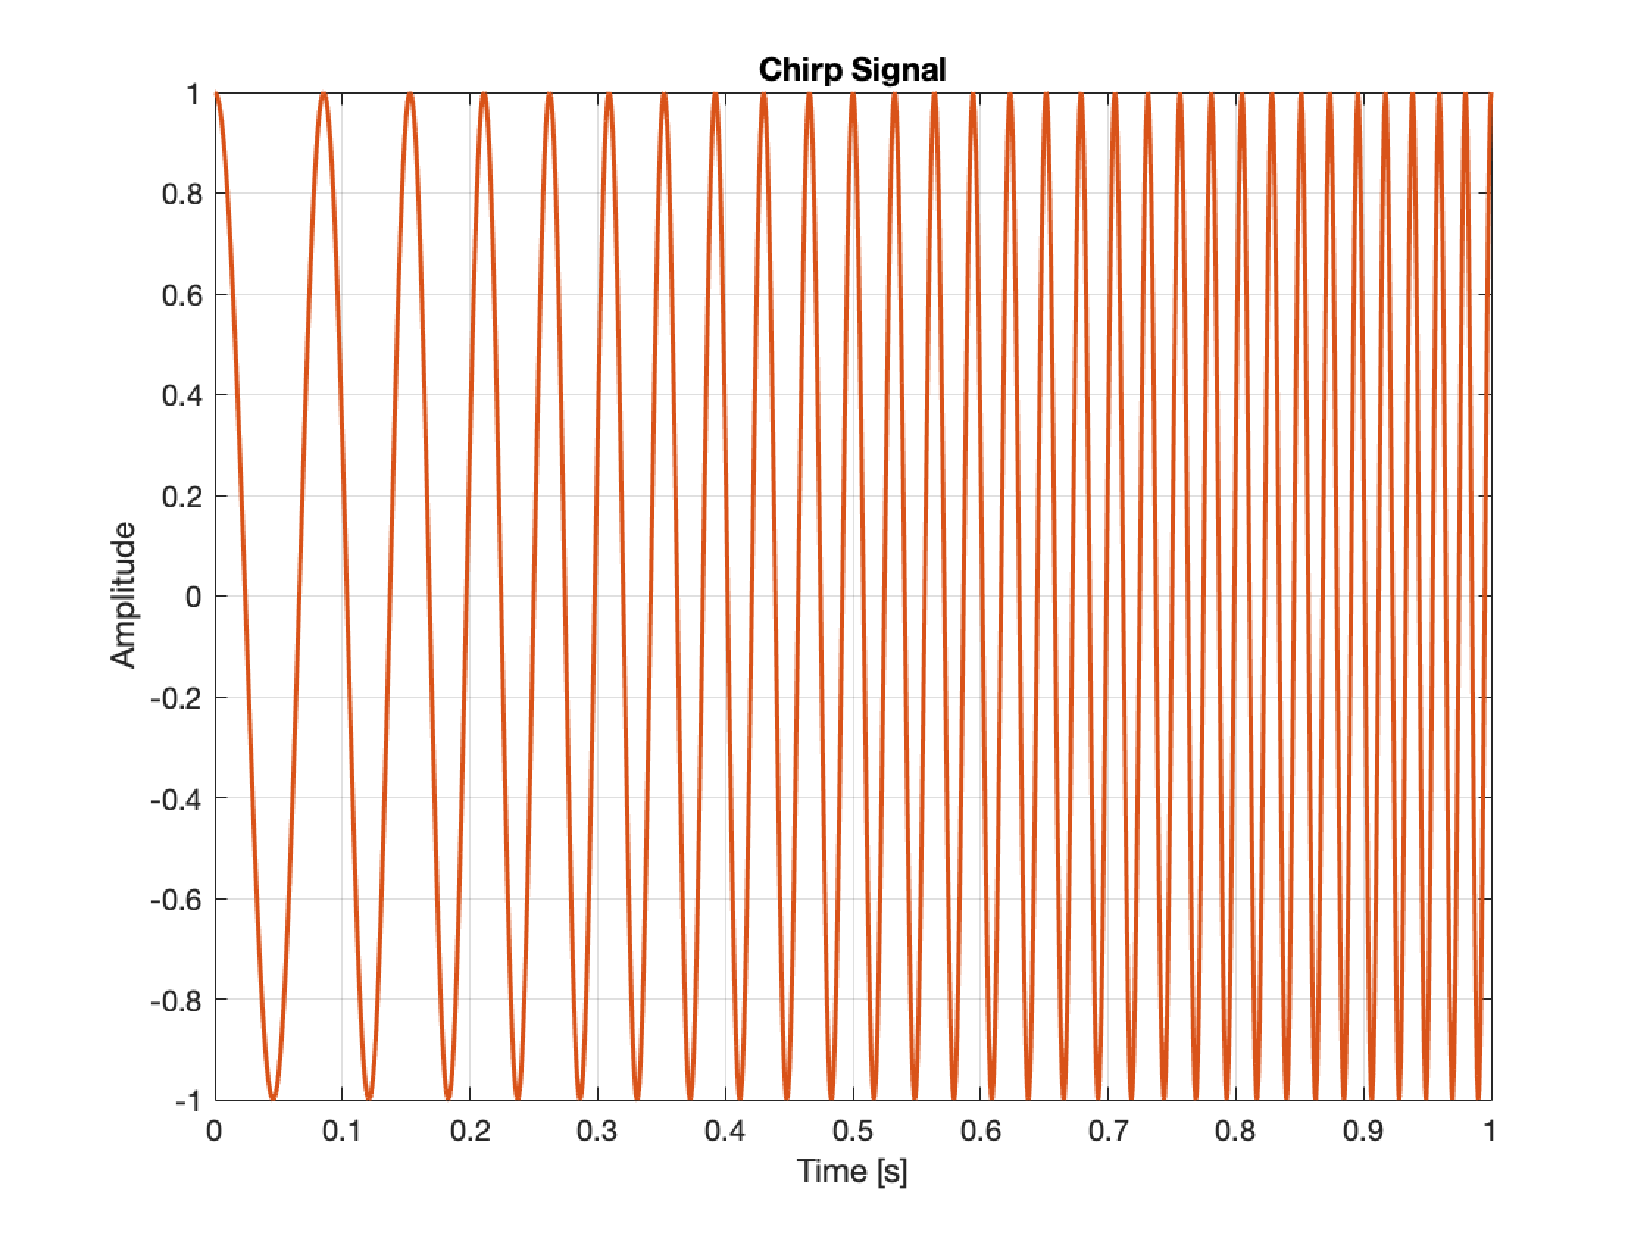
\includegraphics[width = 0.5\textwidth]{images/chirp.pdf}
    \caption{Chirp Signal - Time Domain $1\ Hz$ to $30\ Hz$}\label{chirpTime}
\end{figure}

\begin{figure}[h!]
    \centering
    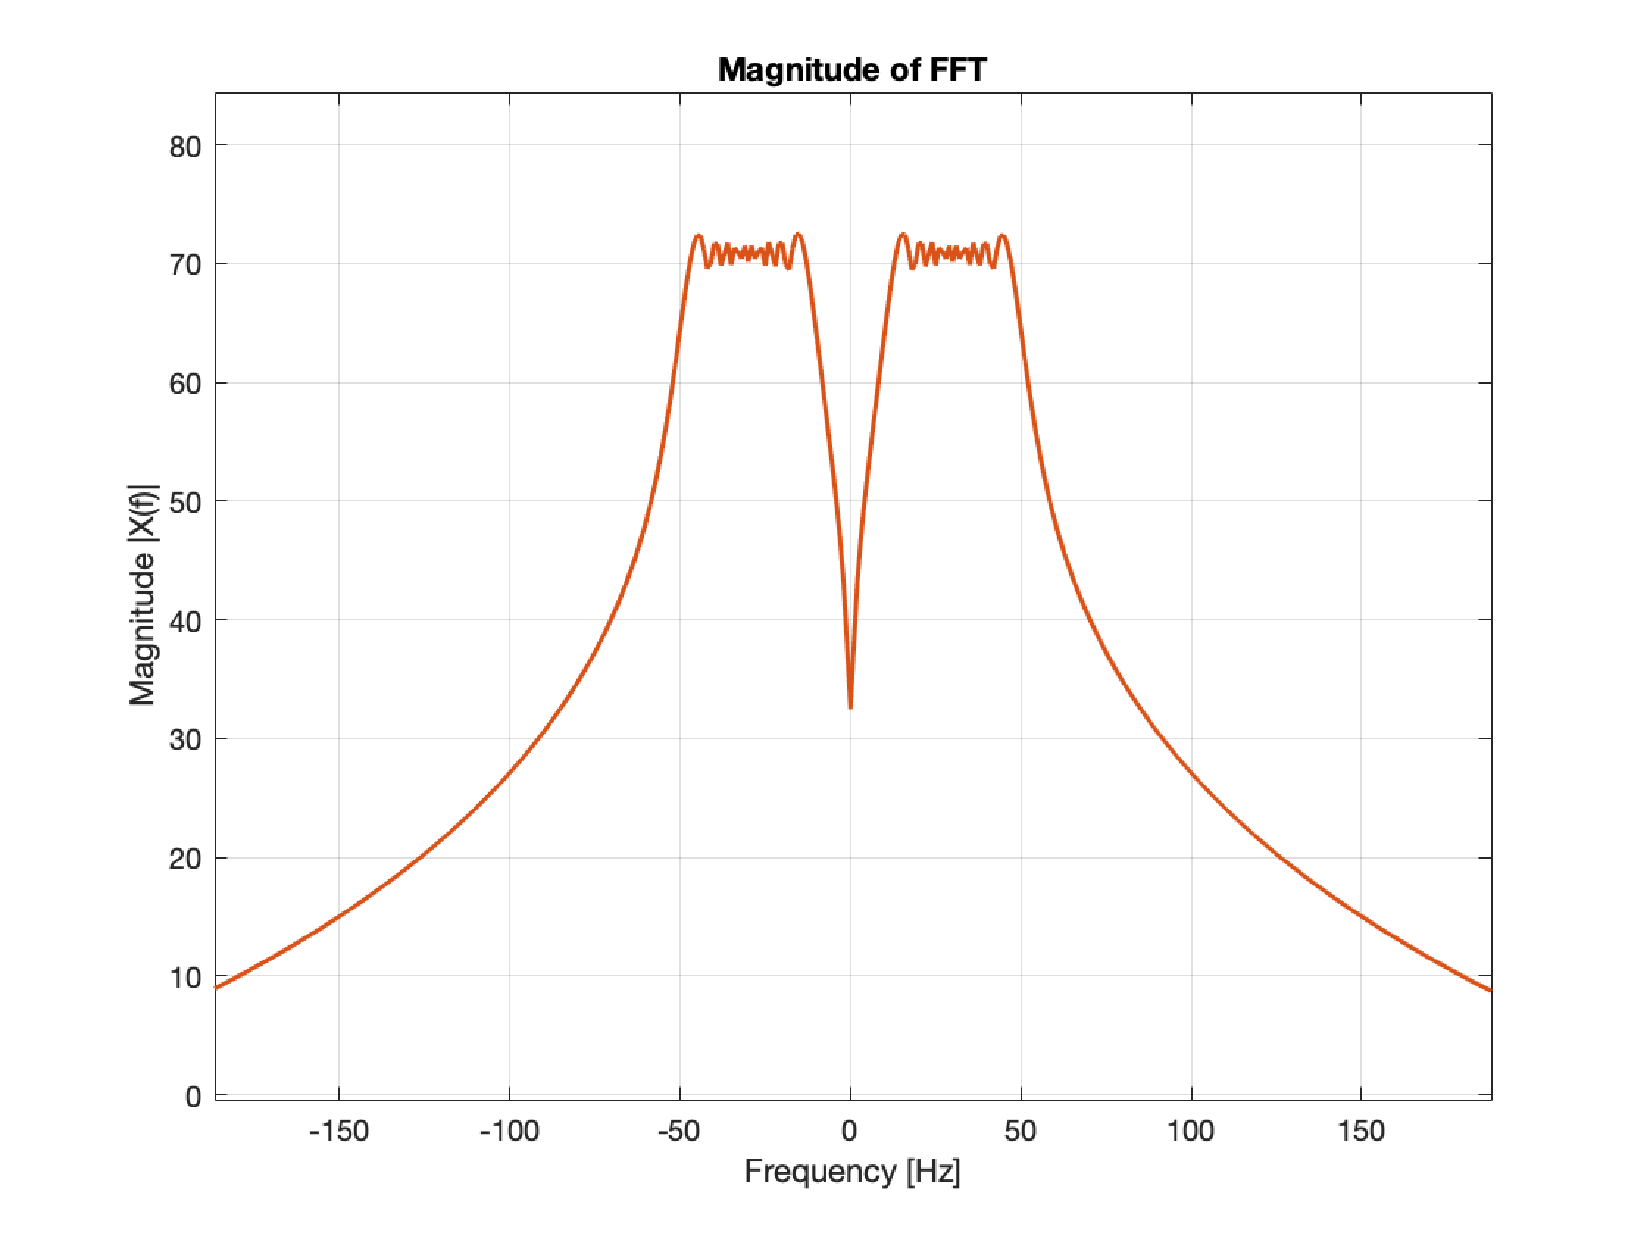
\includegraphics[width = 0.5\textwidth]{images/chirpFFT.pdf}
    \caption{Chirp Signal - Frequency Domain $1\ Hz$ to $30\ Hz$}\label{chirpFFT}
\end{figure}

The above equation results in a signal as seen in Figure \ref{chirpTime} and the FFT of the signal showing the frequency spectrum ranging from $1\ Hz$ to $30\ Hz$ in Figure \ref{chirpFFT}. 
\subsection{Bandwidth}
The bandwidth of the signal can be described as the difference between the higher frequency and the lower frequency in the chirp as depicted in Figure \ref{chirpFFT}.

\section{Waveform Types for Radar Applications}

\subsection{Pulse-Doppler Radar}
Pulse-Doppler radar is when pulses are transmitted at a certain frequency or with a chirp which starts at a specific frequency and goes up to a higher frequency with the bandwidth. A pulse is transmitted after which a listening time where no sound is played. The listening time is used to wait for the echo from the target to return. The distance is then determined by taking into account the time delay from the transmission of the pulse to receiving the echo. Since the speed of sound in air is known, the range of the target can be determined using the formula below. \cite{richards_principles_2010}

\begin{equation}
    R = \frac{t_d c}{2}
\end{equation}{}

Where $R$ is the range of the target, $t_d$ is the time delay before an echo is heard and $c$ is the speed of sound in air.

The Doppler Frequency is used to determine whether or not the target is moving with a radial velocity relative to the radar transmitter. The Doppler Frequency is determined by checking by how much the target has moved over the number of pulses.


\subsection{Continuous Wave (CW)}
Continuous Wave (CW) radar is when a constant frequency tone is played out for a set amount of time or indefinitely and direct measurement of the Doppler shift of the return signal. The wavelength of the returned signal will be different from the transmitted signal. This is known as the Doppler Frequency. CW radars can not be used for range estimation or measurement but only for velocity measurement. There is no basis for measuring the time delay. In Figure \ref{Wavelength} below, the time delay in the wavelength can be seen graphically. \cite{noauthor_continuous_2019}

\begin{figure}[h!]
    \centering
    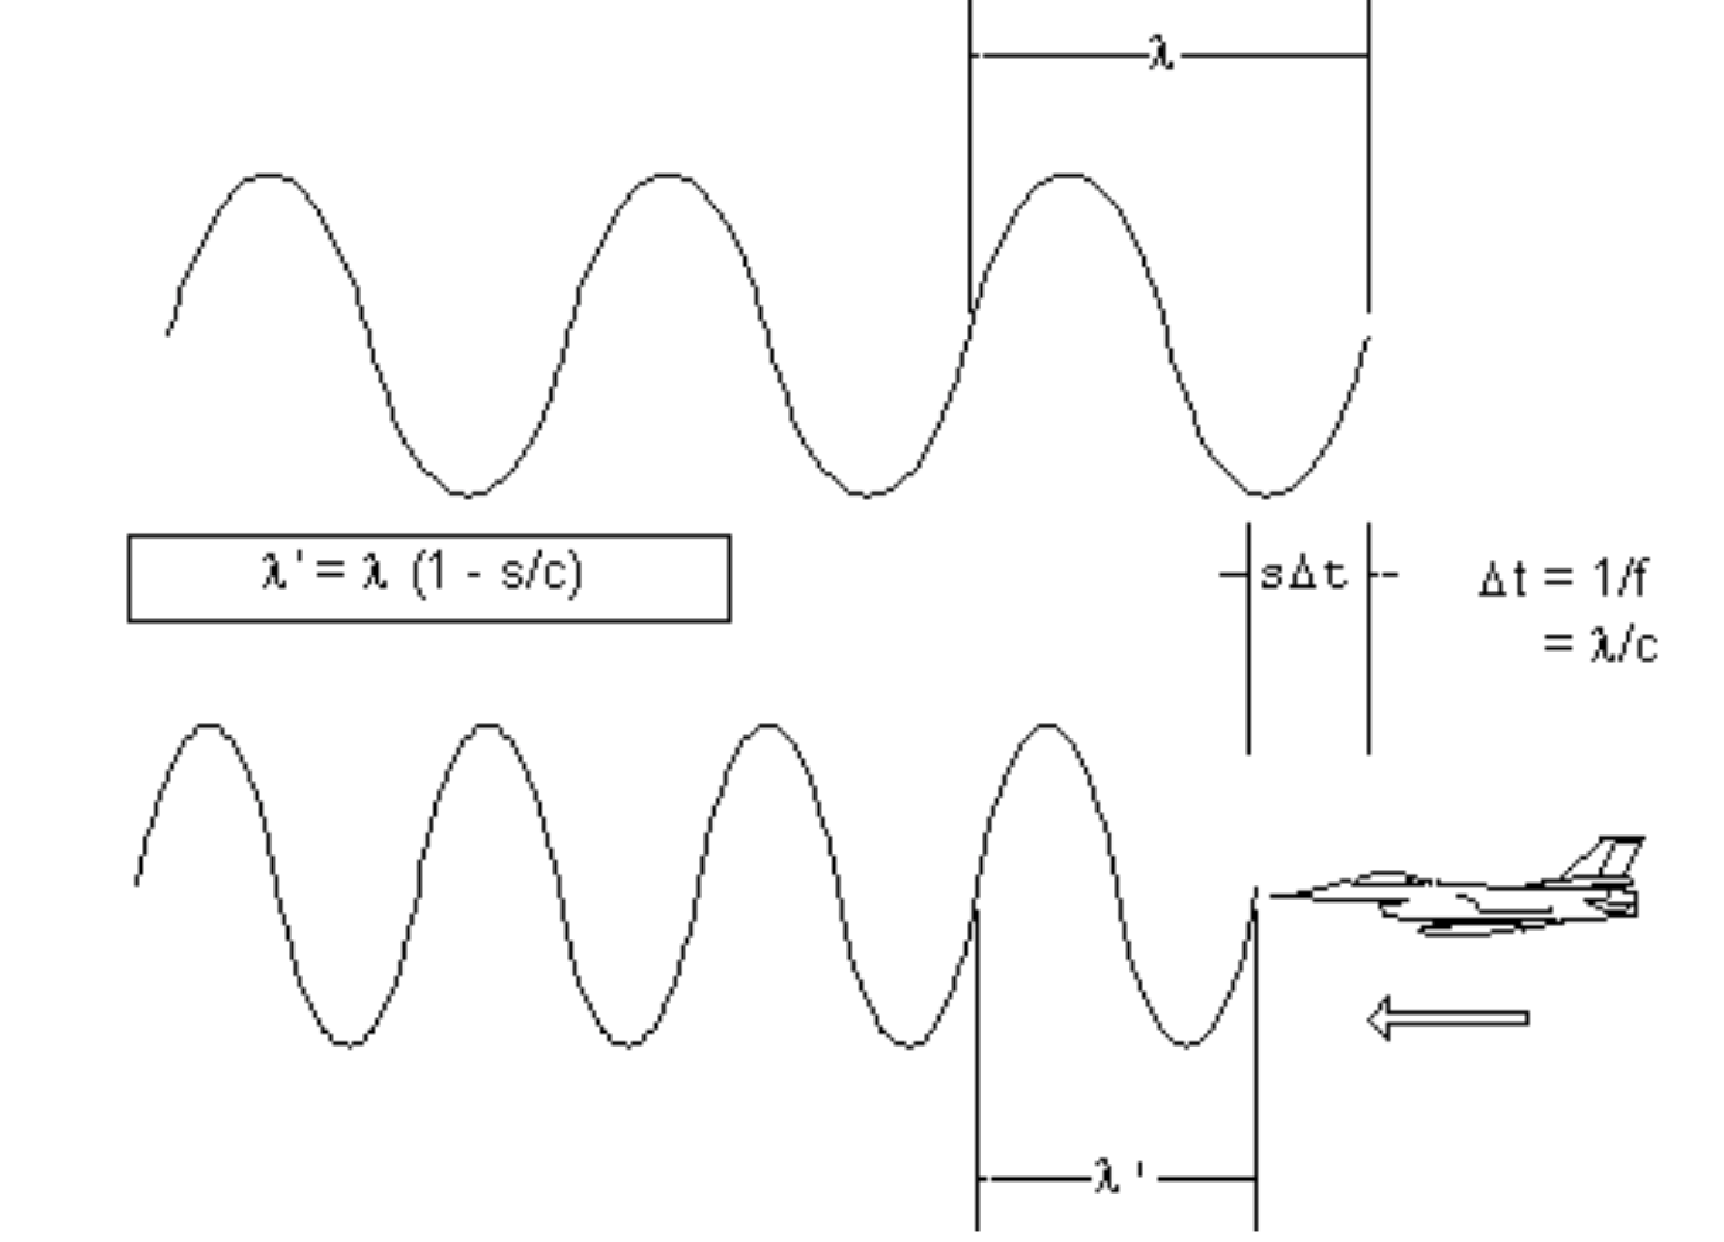
\includegraphics[width = 0.5\textwidth]{images/CW.pdf}
    \caption{Illustration of the Wavelength Change of the Return Signal}\label{Wavelength}
\end{figure}

\subsection{Frequency Modulated Continuous Wave (FMCW)}
Frequency Modulated Continuous Wave (FMCW) radar is used to measure range using the CW radar above but by modulating the frequency. The frequency is varied linearly and the transmitted signal is therefore ‘timestamped’ by the specific frequency that it is at. This timestamp is then used to determine the time delay between transmit and receive and in turn used to calculate the range of the target. The theory can be seen in Figure \ref{FMCW} below. \cite{noauthor_continuous_2019}

\begin{figure}[h!]
    \centering
    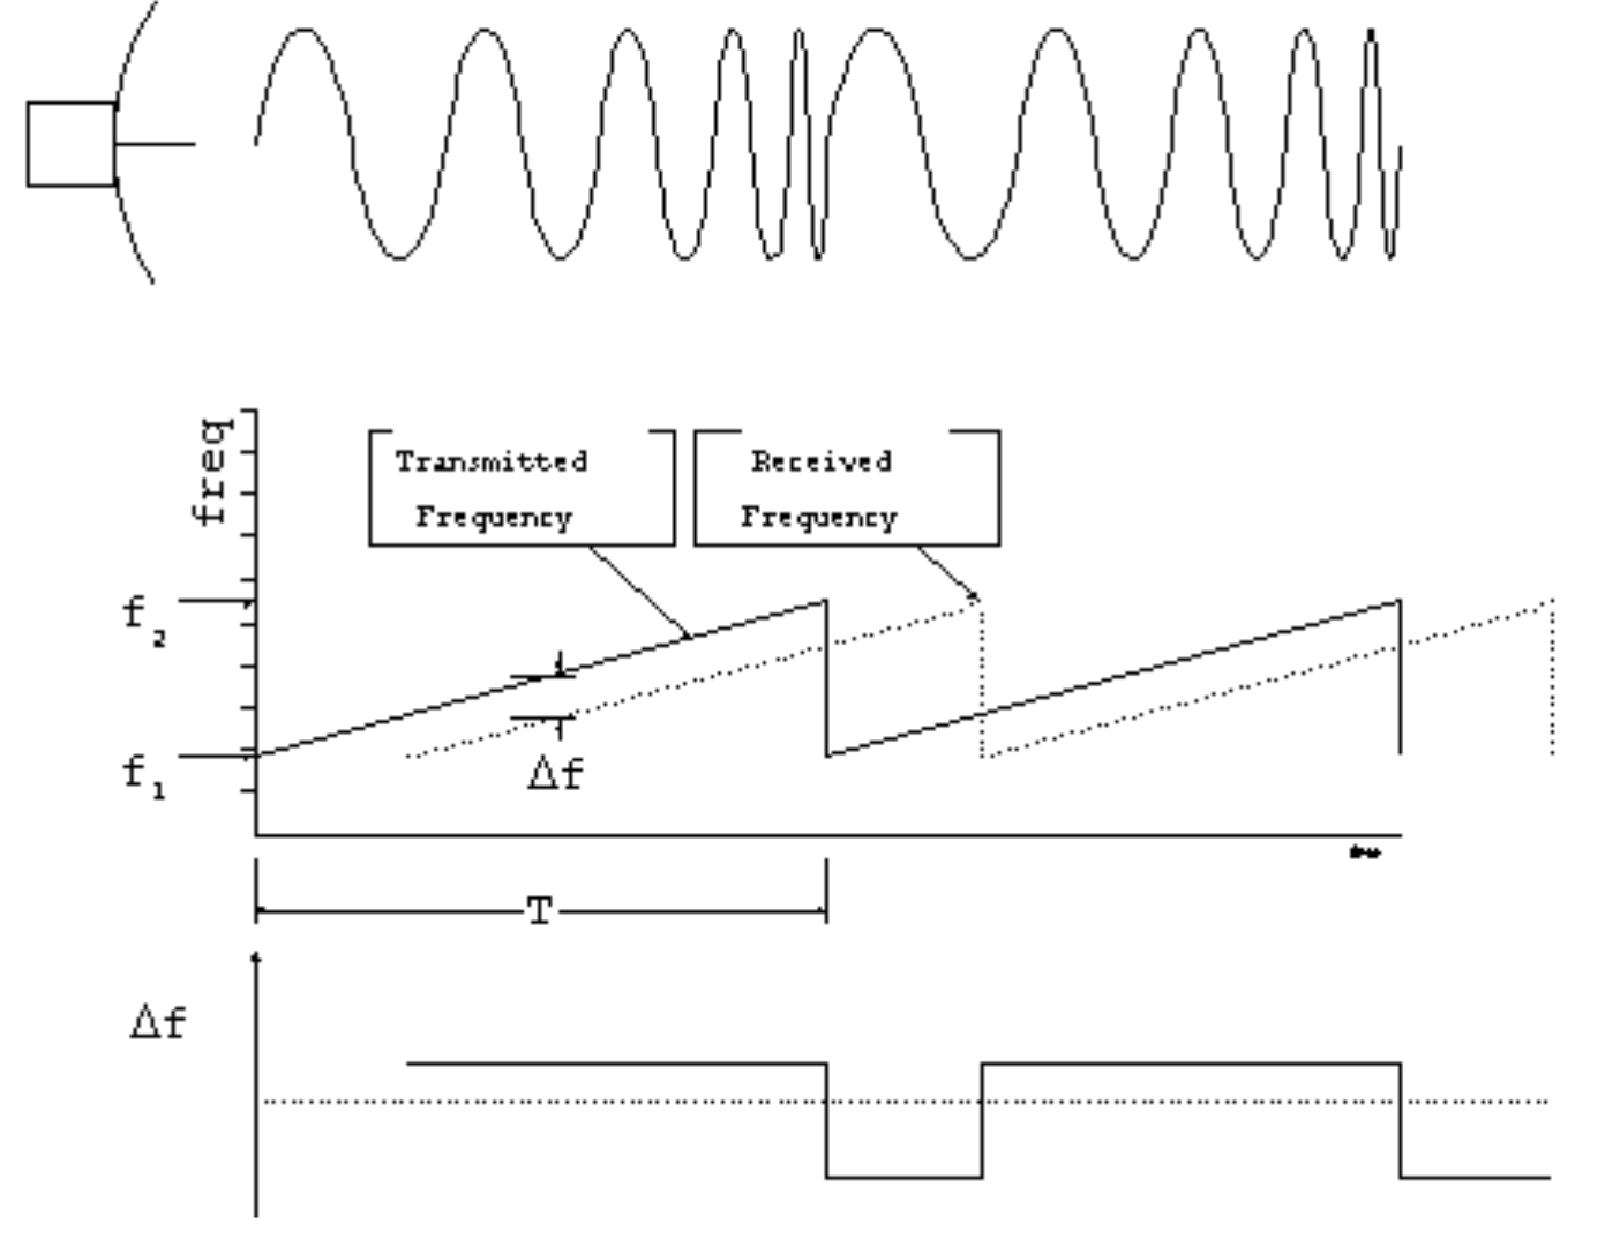
\includegraphics[width = 0.5\textwidth]{images/FMCW.pdf}
    \caption{Illustration of the Frequency Modulation within FMCW}\label{FMCW}
\end{figure}

\section{Windowing Functions\label{window}}
The only windowing function used in the processing of the signals is the Hamming Window. Figure \ref{hamming} shows the time domain plot of a Hamming Windowing function and also the FFT of the signal.
\begin{figure}[h!]
    \centering
    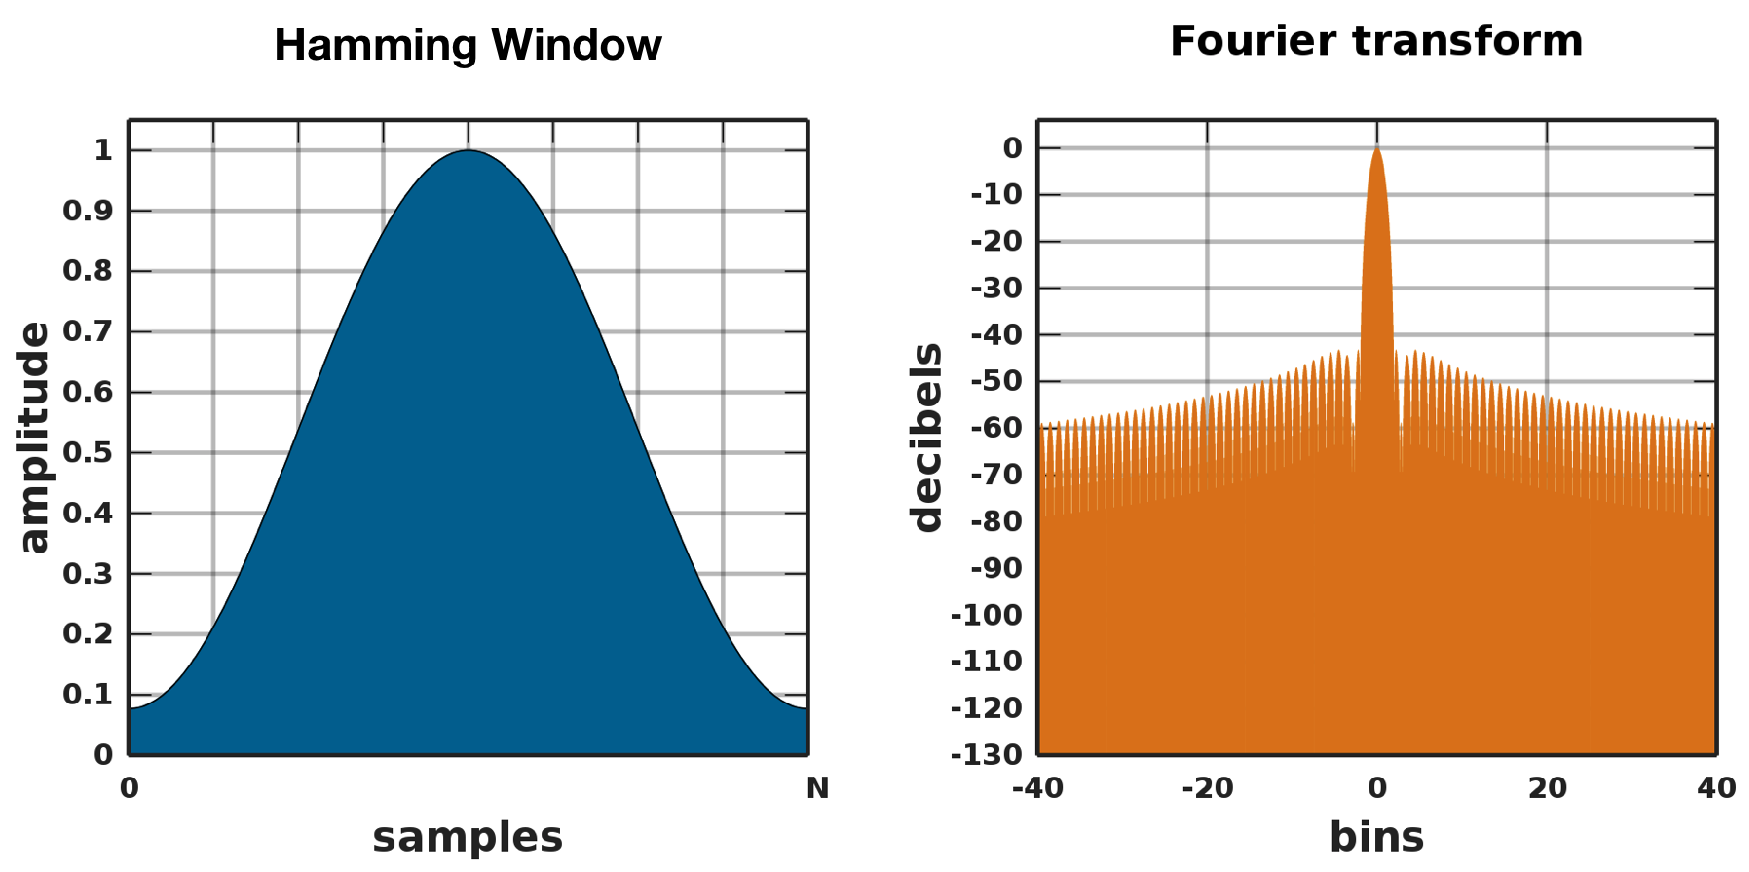
\includegraphics[width = 0.75\textwidth]{images/hamming.pdf}
    \caption{Hamming Windowing function}\label{hamming}\cite{heinzel_spectrum_2002}
\end{figure}
The Normalised Equivalent Noise Bandwidth of the Hamming Windowing function (NENBW) is 1.3628 bins. The theory behind the windowing function would not be investigated since it falls outside the scope of this project. However, it is important to note the windowing function used in the signal processing. The Hamming Window can be obtained using mathematical equation 
\begin{equation}
w[n] = a_0 - (1 - a_0) \cdot cos\Big(\frac{2\pi n}{N}\Big)
\end{equation}
where $a_0\ =\ 0.54$ and this categorises the windowing function as a Hamming Window.

\section{Signal Processing} 
\subsection{Downmixing and Low Pass Filter}

Downmixing of a signal involves the process where the signal is downmixed and the results is a complex version of the signal in its baseband. Sine and cosine waves can be considered the same signal but the cosine signal has a phase shift of $90 °$ from the sine. Multiplying the received signal by sine and cosine at the same centre frequency results in a spectrum with components at $2f_c$ and $-2f_c$ and the added components at $0\ Hz$. Passing the complex signal through a digital low pass filter results in the downmixed signal at baseband in its In-Phase and Quadrature components. An illustration of the entire process can be seen in Figure \ref{fig:downmix} and the theory behind the low pass filter can be seen in Figure \ref{fig:lpfDownmix}.

\begin{figure}[h!]
    \centering
    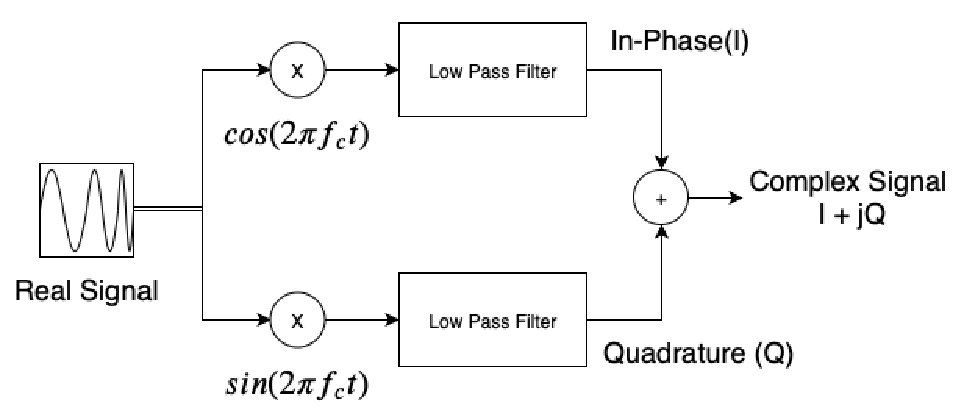
\includegraphics[width = 0.5\textwidth]{images/downmix.pdf}
    \caption{Downmixing Signal to Base band}\label{fig:downmix}
\end{figure}

\begin{figure}[h!]
    \centering
    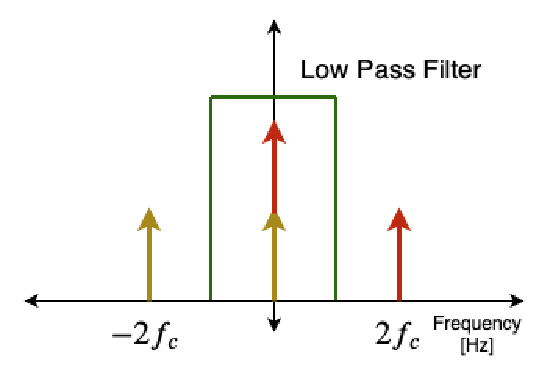
\includegraphics[width = 0.5\textwidth]{images/lpfDownmix.pdf}
    \caption{Low Pass Filter within Downmixing Function}\label{fig:lpfDownmix}
\end{figure}

\subsection{Matched Filter}

A matched filter is the method to increase the signal to noise ratio (SNR) of a received signal. The known transmitted pulse is used to correlate with the received signal. The transmitted pulse is used to detect the presence of the pulse within the unknown received signal. An illustration of the matched filter can be seen in Figure \ref{fig:mfIll}. 

\begin{figure}[h!]
    \centering
    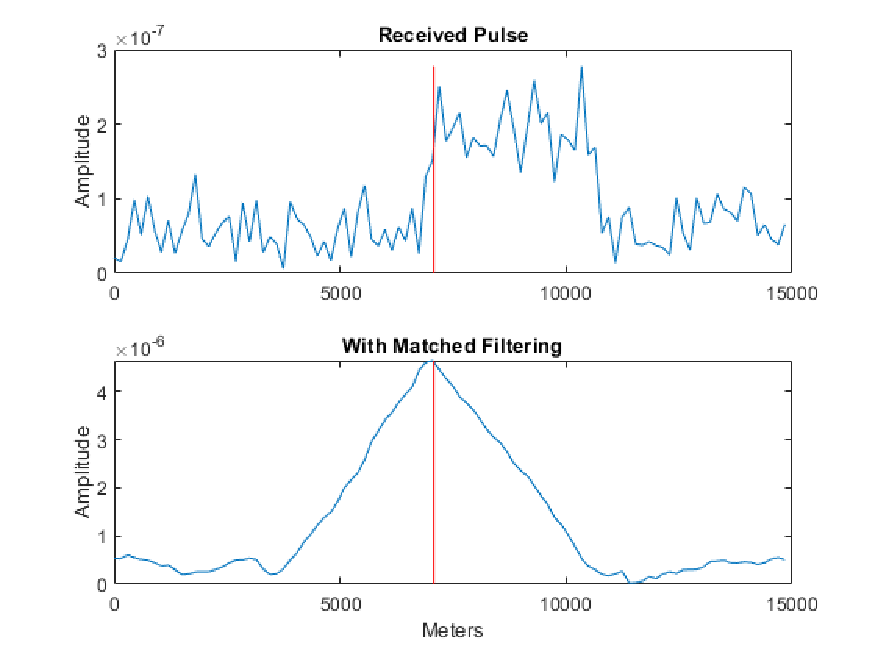
\includegraphics[width = 0.5\textwidth]{images/mfIll.pdf}
    \caption{Illustration of Matched Filter \cite{noauthor_matched_nodate}}\label{fig:mfIll}
\end{figure}

The SNR of the received signal is greatly improved after applying the matched filter making object detection easier. The matched filter improves the probability of detection $P_d\ \approx 90\ \%$ and the probability of false detection $P_{fa}\ \approx\ 10^{-5}$. It is possible for the match filtering to take place in the time domain but the easier implementation is done in the frequency domain as is the case for this system.  

\newpage
\subsection{Range Line vs Time}

The matched filter essentially translates to the range line needed to display the distance to detected targets. The array containing all of the range data is currently in a vector form and the vector needs to be broken up into the different number of pulses that were played out initially. The \verb np.reshape()  function is used to reshape the vector into a matrix of shape $n$ x $m$ where $n$ is the rows consisting of the number of pulses and $m$ is the range measured to the target. The general function of going from the rangeline to a matrix is illustrated in Figure \ref{fig:rangeline2Matrix}.

\begin{figure}[h!]
    \centering
    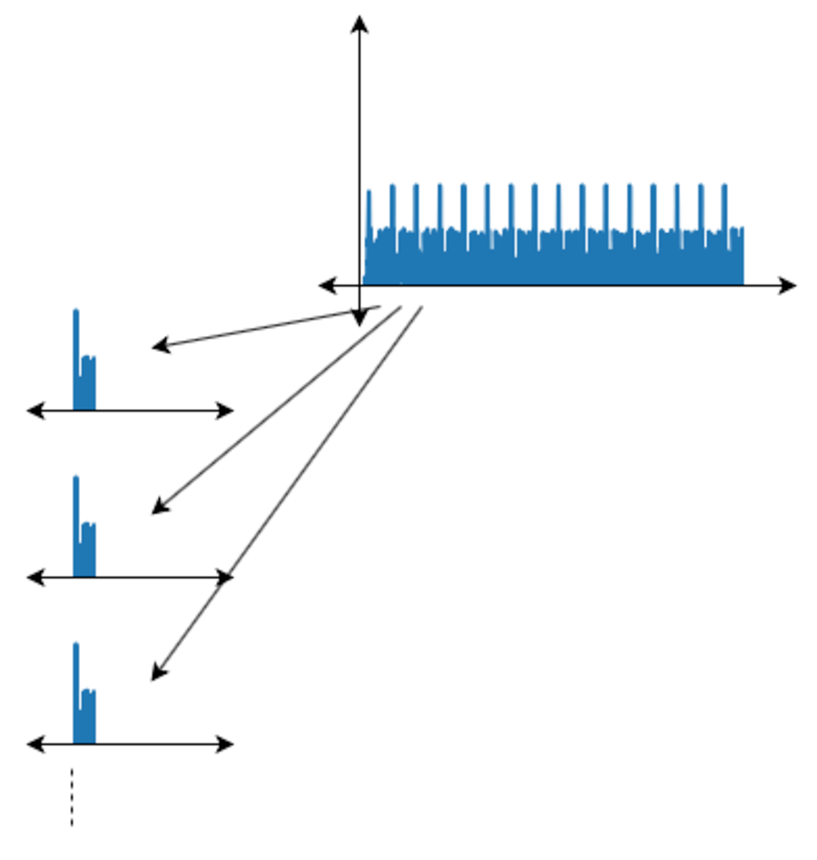
\includegraphics[width = 0.45\textwidth]{images/rangeline2Matrix.pdf}
    \caption{Illustration of Rangeline to Range Matrix}\label{fig:rangeline2Matrix}
\end{figure}

\newpage